\documentclass[10pt, a4paper, english]{article}\usepackage[]{graphicx}\usepackage[dvipsnames]{xcolor}
% maxwidth is the original width if it is less than linewidth
% otherwise use linewidth (to make sure the graphics do not exceed the margin)
\makeatletter
\def\maxwidth{ %
  \ifdim\Gin@nat@width>\linewidth
    \linewidth
  \else
    \Gin@nat@width
  \fi
}
\makeatother

\definecolor{fgcolor}{rgb}{0.345, 0.345, 0.345}
\newcommand{\hlnum}[1]{\textcolor[rgb]{0.686,0.059,0.569}{#1}}%
\newcommand{\hlstr}[1]{\textcolor[rgb]{0.192,0.494,0.8}{#1}}%
\newcommand{\hlcom}[1]{\textcolor[rgb]{0.678,0.584,0.686}{\textit{#1}}}%
\newcommand{\hlopt}[1]{\textcolor[rgb]{0,0,0}{#1}}%
\newcommand{\hlstd}[1]{\textcolor[rgb]{0.345,0.345,0.345}{#1}}%
\newcommand{\hlkwa}[1]{\textcolor[rgb]{0.161,0.373,0.58}{\textbf{#1}}}%
\newcommand{\hlkwb}[1]{\textcolor[rgb]{0.69,0.353,0.396}{#1}}%
\newcommand{\hlkwc}[1]{\textcolor[rgb]{0.333,0.667,0.333}{#1}}%
\newcommand{\hlkwd}[1]{\textcolor[rgb]{0.737,0.353,0.396}{\textbf{#1}}}%
\let\hlipl\hlkwb

\usepackage{framed}
\makeatletter
\newenvironment{kframe}{%
 \def\at@end@of@kframe{}%
 \ifinner\ifhmode%
  \def\at@end@of@kframe{\end{minipage}}%
  \begin{minipage}{\columnwidth}%
 \fi\fi%
 \def\FrameCommand##1{\hskip\@totalleftmargin \hskip-\fboxsep
 \colorbox{shadecolor}{##1}\hskip-\fboxsep
     % There is no \\@totalrightmargin, so:
     \hskip-\linewidth \hskip-\@totalleftmargin \hskip\columnwidth}%
 \MakeFramed {\advance\hsize-\width
   \@totalleftmargin\z@ \linewidth\hsize
   \@setminipage}}%
 {\par\unskip\endMakeFramed%
 \at@end@of@kframe}
\makeatother

\definecolor{shadecolor}{rgb}{.97, .97, .97}
\definecolor{messagecolor}{rgb}{0, 0, 0}
\definecolor{warningcolor}{rgb}{1, 0, 1}
\definecolor{errorcolor}{rgb}{1, 0, 0}
\newenvironment{knitrout}{}{} % an empty environment to be redefined in TeX

\usepackage{alltt}
%typesetting
\usepackage[margin = 1in]{geometry} % margins
\usepackage[T1]{fontenc} % font encoding
\usepackage{babel} %enables typesetting for multiple languages
\usepackage{parskip} %new lines
\usepackage{graphicx} 
\usepackage{float}
\floatplacement{figure}{H} %when printing tables, include  table.position="H"
\usepackage{bm}
\usepackage{amsmath}

\usepackage[dvipsnames]{xcolor} % more colors

\usepackage[colorlinks]{hyperref}


 %clickable table of contents from hyperref
\hypersetup{
    colorlinks,
    citecolor=black,
    filecolor=black,
    linkcolor=black,
    urlcolor=black
}

\usepackage[colorinlistoftodos]{todonotes}

\title{Machine Learning 2ST129 26605 HT2023
 Assignment 8}
\author{Anonymous Student}
\date{\today}
\IfFileExists{upquote.sty}{\usepackage{upquote}}{}
\begin{document}
\maketitle
\newpage
\tableofcontents
\newpage

\section*{General Information}
\addcontentsline{toc}{section}{General Information}
\begin{itemize}
\item Time used for reading 3 hours: 
\item Time used for basic assignment 14 hours:
\item Time used for extra assignment NA: 
\item Good with lab: It was fun to implement different algorithms and see how they performed. Also i felt that i learned the basic idea of reinforcement learning.
\item Things improve with lab: Not necessarily an improvement, but I think it could have been fun to implement some larger task rather than just many smaller tasks and have to task  focused to be  more of a program rather than just some individual functions. 
\end{itemize}

\newpage


\begin{knitrout}
\definecolor{shadecolor}{rgb}{0.969, 0.969, 0.969}\color{fgcolor}\begin{kframe}
\begin{alltt}
\hlcom{#Libraries}
 \hlkwd{library}\hlstd{(tidyverse)}
 \hlkwd{library}\hlstd{(xtable)}
 \hlkwd{library}\hlstd{(tensorflow)}
 \hlkwd{library}\hlstd{(keras)}
\end{alltt}
\end{kframe}
\end{knitrout}

\section{Task 1: Bandits}
\subsection{Task 1.1: stationary bandits}
 Here we implement a stationary bandit function,  which takes an action and returns a reward. The reward is sampled from a normal distribution with mean $\mu = q^*_a$ and standard deviation $\sigma = 1$ and where $q^*_a = (1-62, 1.2, 0.7, 0.72, 2.03)$.

\begin{knitrout}
\definecolor{shadecolor}{rgb}{0.969, 0.969, 0.969}\color{fgcolor}\begin{kframe}
\begin{alltt}
\hlcom{#do the same as staionary bandit but check that a is an integer between 1 and 5}
\hlstd{stationary_bandit} \hlkwb{<-} \hlkwa{function}\hlstd{(}\hlkwc{a}\hlstd{,} \hlkwc{t}\hlstd{=}\hlkwa{NULL}\hlstd{)\{}
  \hlstd{q_star} \hlkwb{<-} \hlkwd{c}\hlstd{(}\hlnum{1.62}\hlstd{,} \hlnum{1.2}\hlstd{,} \hlnum{0.7}\hlstd{,} \hlnum{0.72}\hlstd{,} \hlnum{2.03}\hlstd{)}
  \hlkwa{if}\hlstd{(a} \hlopt \hlnum{1}\hlopt{:}\hlnum{5}\hlstd{)\{}
    \hlstd{reward} \hlkwb{<-} \hlkwd{rnorm}\hlstd{(}\hlnum{1}\hlstd{,} \hlkwc{mean} \hlstd{= q_star[a],} \hlkwc{sd} \hlstd{=} \hlnum{1}\hlstd{)}
    \hlkwd{return}\hlstd{(reward)}
  \hlstd{\}} \hlkwa{else}\hlstd{\{}
    \hlkwd{print}\hlstd{(}\hlstr{"a must be an integer between 1 and 5"}\hlstd{)}
  \hlstd{\}}
\hlstd{\}}
\end{alltt}
\end{kframe}
\end{knitrout}
 
\begin{knitrout}
\definecolor{shadecolor}{rgb}{0.969, 0.969, 0.969}\color{fgcolor}\begin{kframe}
\begin{alltt}
\hlcom{#test the function}
\hlkwd{set.seed}\hlstd{(}\hlnum{4711}\hlstd{)}
\hlkwd{stationary_bandit}\hlstd{(}\hlnum{2}\hlstd{)}
\end{alltt}
\begin{verbatim}
[1] 3.019735
\end{verbatim}
\begin{alltt}
\hlkwd{stationary_bandit}\hlstd{(}\hlnum{1}\hlstd{)}
\end{alltt}
\begin{verbatim}
[1] 2.99044
\end{verbatim}
\begin{alltt}
\hlstd{R} \hlkwb{<-} \hlkwd{numeric}\hlstd{(}\hlnum{1000}\hlstd{)}
\hlkwa{for}\hlstd{(i} \hlkwa{in} \hlnum{1}\hlopt{:} \hlnum{1000}\hlstd{)\{}
  \hlstd{R[i]} \hlkwb{<-} \hlkwd{stationary_bandit}\hlstd{(}\hlnum{3}\hlstd{)}
\hlstd{\}}
\hlkwd{mean}\hlstd{(R)}
\end{alltt}
\begin{verbatim}
[1] 0.6819202
\end{verbatim}
\end{kframe}
\end{knitrout}
 
\subsection{Task 1.2: non-stationary bandits}
Next we implement a non-stationary bandit function. For all actions 2 to 5, it works as the stationary reward function, but for a = 1 it returns a reward based on normal(-3 +0.01t, 1).
\begin{knitrout}
\definecolor{shadecolor}{rgb}{0.969, 0.969, 0.969}\color{fgcolor}\begin{kframe}
\begin{alltt}
\hlstd{nonstationary_bandit} \hlkwb{<-} \hlkwa{function}\hlstd{(}\hlkwc{a}\hlstd{,} \hlkwc{t}\hlstd{)\{}
  \hlstd{q_star} \hlkwb{<-} \hlkwd{c}\hlstd{(}\hlnum{1.62}\hlstd{,} \hlnum{1.2}\hlstd{,} \hlnum{0.7}\hlstd{,} \hlnum{0.72}\hlstd{,} \hlnum{2.03}\hlstd{)}
  \hlkwa{if}\hlstd{(a} \hlopt \hlnum{1}\hlopt{:}\hlnum{5}\hlstd{)\{}
    \hlkwa{if}\hlstd{(a} \hlopt{==} \hlnum{1}\hlstd{)\{}
      \hlstd{reward} \hlkwb{<-} \hlkwd{rnorm}\hlstd{(}\hlnum{1}\hlstd{,} \hlkwc{mean} \hlstd{=} \hlopt{-}\hlnum{3} \hlopt{+} \hlnum{0.01}\hlopt{*}\hlstd{t,} \hlkwc{sd} \hlstd{=} \hlnum{1}\hlstd{)}
      \hlkwd{return}\hlstd{(reward)}
    \hlstd{\}} \hlkwa{else}\hlstd{\{}
      \hlstd{reward} \hlkwb{<-} \hlkwd{rnorm}\hlstd{(}\hlnum{1}\hlstd{,} \hlkwc{mean} \hlstd{= q_star[a],} \hlkwc{sd} \hlstd{=} \hlnum{1}\hlstd{)}
      \hlkwd{return}\hlstd{(reward)}
    \hlstd{\}}
  \hlstd{\}} \hlkwa{else}\hlstd{\{}
    \hlkwd{print}\hlstd{(}\hlstr{"a must be an integer between 1 and 5"}\hlstd{)}
  \hlstd{\}}
\hlstd{\}}
\end{alltt}
\end{kframe}
\end{knitrout}
 
\begin{knitrout}
\definecolor{shadecolor}{rgb}{0.969, 0.969, 0.969}\color{fgcolor}\begin{kframe}
\begin{alltt}
\hlkwd{set.seed}\hlstd{(}\hlnum{4711}\hlstd{)}
\hlkwd{nonstationary_bandit}\hlstd{(}\hlnum{2}\hlstd{,} \hlkwc{t} \hlstd{=} \hlnum{1}\hlstd{)}
\end{alltt}
\begin{verbatim}
[1] 3.019735
\end{verbatim}
\begin{alltt}
\hlkwd{nonstationary_bandit}\hlstd{(}\hlnum{2}\hlstd{,} \hlkwc{t} \hlstd{=} \hlnum{1000}\hlstd{)}
\end{alltt}
\begin{verbatim}
[1] 2.57044
\end{verbatim}
\begin{alltt}
\hlkwd{nonstationary_bandit}\hlstd{(}\hlnum{1}\hlstd{,} \hlkwc{t} \hlstd{=} \hlnum{1}\hlstd{)}
\end{alltt}
\begin{verbatim}
[1] -1.793682
\end{verbatim}
\begin{alltt}
\hlkwd{nonstationary_bandit}\hlstd{(}\hlnum{1}\hlstd{,} \hlkwc{t} \hlstd{=} \hlnum{1000}\hlstd{)}
\end{alltt}
\begin{verbatim}
[1] 6.593121
\end{verbatim}
\end{kframe}
\end{knitrout}
 
\subsection{Task 1.3:  greedy algorithm}
 Here we implement a greedy algorithm that always chooses the greedy action according to the equation: $A_t \doteq \underset{a}{\operatorname{argmax}} Q_t(a)$. The function takes a vector of initial estimates $Q_1$ and a reward function, and then run the bandit for 1000 steps and return four things: the rewards $R_t$ for all steps, the mean reward for all 1000 steps, the value estimates $Q_t(a)$ and the total number of choices of each action, $Nt(a)$.
\begin{knitrout}
\definecolor{shadecolor}{rgb}{0.969, 0.969, 0.969}\color{fgcolor}\begin{kframe}
\begin{alltt}
\hlstd{greedy_algorithm} \hlkwb{<-} \hlkwa{function}\hlstd{(}\hlkwc{Q1}\hlstd{,} \hlkwc{bandit}\hlstd{,} \hlkwc{n_steps} \hlstd{=} \hlnum{1000}\hlstd{) \{}
  \hlstd{num_actions} \hlkwb{<-} \hlkwd{length}\hlstd{(Q1)}
  \hlstd{all_rewards} \hlkwb{<-} \hlkwd{numeric}\hlstd{(n_steps)}
  \hlstd{Q_t} \hlkwb{<-} \hlkwd{numeric}\hlstd{(num_actions)}
  \hlstd{N_t} \hlkwb{<-} \hlkwd{rep}\hlstd{(}\hlnum{0}\hlstd{, num_actions)}

  \hlkwa{for} \hlstd{(t} \hlkwa{in} \hlnum{1}\hlopt{:}\hlstd{n_steps) \{}
    \hlstd{action_t} \hlkwb{<-} \hlkwd{which.max}\hlstd{(Q1)}

    \hlkwa{if} \hlstd{(}\hlkwd{identical}\hlstd{(bandit, stationary_bandit)) \{}
      \hlstd{reward_t} \hlkwb{<-} \hlkwd{stationary_bandit}\hlstd{(action_t)}
    \hlstd{\}} \hlkwa{else if} \hlstd{(}\hlkwd{identical}\hlstd{(bandit, nonstationary_bandit)) \{}
      \hlstd{reward_t} \hlkwb{<-} \hlkwd{nonstationary_bandit}\hlstd{(action_t, t)}
    \hlstd{\}} \hlkwa{else} \hlstd{\{}
      \hlkwd{stop}\hlstd{(}\hlstr{"Invalid bandit function"}\hlstd{)}
    \hlstd{\}}

    \hlcom{# Update estimates}
    \hlstd{N_t[action_t]} \hlkwb{<-} \hlstd{N_t[action_t]} \hlopt{+} \hlnum{1}
    \hlstd{Q1[action_t]} \hlkwb{<-} \hlstd{Q1[action_t]} \hlopt{+} \hlstd{(reward_t} \hlopt{-} \hlstd{Q1[action_t])} \hlopt{/} \hlstd{N_t[action_t]}

    \hlcom{# Save reward}
    \hlstd{all_rewards[t]} \hlkwb{<-} \hlstd{reward_t}
    \hlstd{Q_t[action_t]} \hlkwb{<-} \hlstd{Q1[action_t]}
  \hlstd{\}}

  \hlstd{mean_reward} \hlkwb{<-} \hlkwd{mean}\hlstd{(all_rewards)}

  \hlkwd{return}\hlstd{(}\hlkwd{list}\hlstd{(}\hlkwc{Qt} \hlstd{= Q_t,} \hlkwc{Nt} \hlstd{= N_t,} \hlkwc{R_bar} \hlstd{= mean_reward,} \hlkwc{Rt} \hlstd{= all_rewards))}
\hlstd{\}}
\end{alltt}
\end{kframe}
\end{knitrout}

\begin{knitrout}
\definecolor{shadecolor}{rgb}{0.969, 0.969, 0.969}\color{fgcolor}\begin{kframe}
\begin{alltt}
\hlkwd{set.seed}\hlstd{(}\hlnum{4711}\hlstd{)}
\hlstd{Q1} \hlkwb{<-} \hlkwd{rep}\hlstd{(}\hlnum{0}\hlstd{,} \hlnum{5}\hlstd{)}
\hlkwd{lapply}\hlstd{(}\hlkwd{greedy_algorithm}\hlstd{(Q1, stationary_bandit), head)}
\end{alltt}
\begin{verbatim}
$Qt
[1] 1.602744 0.000000 0.000000 0.000000 0.000000

$Nt
[1] 1000    0    0    0    0

$R_bar
[1] 1.602744

$Rt
[1] 3.439735 2.990440 2.816318 1.213121 1.009021 0.111088
\end{verbatim}
\end{kframe}
\end{knitrout}

\subsection{Task 1.4: $\epsilon$-greedy algorithm}
Now we implement an $\epsilon$-greedy algorithm that chooses the greedy action with probability $1-\epsilon$ and a random action with probability $\epsilon$. It is based on the same greedy algorithm as before, but now  the parameter \texttt{espilon} is included as an argument. 

\begin{knitrout}
\definecolor{shadecolor}{rgb}{0.969, 0.969, 0.969}\color{fgcolor}\begin{kframe}
\begin{alltt}
\hlstd{epsilon_algorithm} \hlkwb{<-} \hlkwa{function}\hlstd{(}\hlkwc{Q1}\hlstd{,} \hlkwc{bandit}\hlstd{,} \hlkwc{epsilon}\hlstd{,} \hlkwc{n_steps}\hlstd{=}\hlnum{1000}\hlstd{) \{}
  \hlcom{#instantiating initial variables}
  \hlstd{num_actions} \hlkwb{<-} \hlkwd{length}\hlstd{(Q1)}
  \hlstd{all_rewards} \hlkwb{<-} \hlkwd{numeric}\hlstd{(n_steps)}
  \hlstd{Q_t} \hlkwb{<-} \hlkwd{numeric}\hlstd{(num_actions)}
  \hlstd{N_t} \hlkwb{<-}\hlkwd{rep}\hlstd{(}\hlnum{0}\hlstd{, num_actions)}

  \hlkwa{for} \hlstd{(t} \hlkwa{in} \hlnum{1}\hlopt{:}\hlstd{n_steps) \{}
    \hlkwa{if} \hlstd{(}\hlkwd{runif}\hlstd{(}\hlnum{1}\hlstd{)} \hlopt{<} \hlstd{epsilon) \{}
      \hlstd{action_t} \hlkwb{<-} \hlkwd{sample}\hlstd{(}\hlnum{1}\hlopt{:}\hlstd{num_actions,} \hlnum{1}\hlstd{)}
    \hlstd{\}} \hlkwa{else} \hlstd{\{}
      \hlstd{action_t} \hlkwb{<-} \hlkwd{which.max}\hlstd{(Q1)}
    \hlstd{\}}

     \hlkwa{if} \hlstd{(}\hlkwd{identical}\hlstd{(bandit, stationary_bandit)) \{}
      \hlstd{reward_t} \hlkwb{<-} \hlkwd{stationary_bandit}\hlstd{(action_t)}
    \hlstd{\}} \hlkwa{else if} \hlstd{(}\hlkwd{identical}\hlstd{(bandit, nonstationary_bandit)) \{}
      \hlstd{reward_t} \hlkwb{<-} \hlkwd{nonstationary_bandit}\hlstd{(action_t, t)}
    \hlstd{\}} \hlkwa{else} \hlstd{\{}
      \hlkwd{stop}\hlstd{(}\hlstr{"Invalid bandit function"}\hlstd{)}
    \hlstd{\}}

    \hlcom{# Update estimates and save reward}
    \hlstd{N_t[action_t]} \hlkwb{<-} \hlstd{N_t[action_t]} \hlopt{+} \hlnum{1}
    \hlstd{Q1[action_t]} \hlkwb{<-} \hlstd{Q1[action_t]} \hlopt{+} \hlstd{(reward_t} \hlopt{-} \hlstd{Q1[action_t])} \hlopt{/} \hlstd{N_t[action_t]}

    \hlstd{all_rewards[t]} \hlkwb{<-} \hlstd{reward_t}
    \hlstd{Q_t[action_t]} \hlkwb{<-} \hlstd{Q1[action_t]}
  \hlstd{\}}

  \hlstd{mean_reward} \hlkwb{<-} \hlkwd{mean}\hlstd{(all_rewards)}

  \hlkwd{return}\hlstd{(}\hlkwd{list}\hlstd{(}\hlkwc{Qt} \hlstd{= Q_t,} \hlkwc{Nt} \hlstd{= N_t,} \hlkwc{R_bar} \hlstd{= mean_reward,} \hlkwc{R_t} \hlstd{= all_rewards))}
\hlstd{\}}
\hlkwd{set.seed}\hlstd{(}\hlnum{4711}\hlstd{)}
\hlstd{Q1} \hlkwb{<-} \hlkwd{rep}\hlstd{(}\hlnum{0}\hlstd{,} \hlnum{5}\hlstd{)}
\hlkwd{lapply}\hlstd{(}\hlkwd{epsilon_algorithm}\hlstd{(Q1, stationary_bandit,} \hlkwc{epsilon} \hlstd{=} \hlnum{0.1}\hlstd{), head)}
\end{alltt}
\begin{verbatim}
$Qt
[1] 1.6093183 1.1491153 0.7382012 0.5975228 2.0272784

$Nt
[1] 234  17  19  16 714

$R_bar
[1] 1.867178

$R_t
[1] 1.7725176 2.8163182 0.6335086 2.0175494 0.1021861 2.0943547
\end{verbatim}
\begin{alltt}
\hlkwd{set.seed}\hlstd{(}\hlnum{4712}\hlstd{)}
\hlstd{Q1} \hlkwb{<-} \hlkwd{rep}\hlstd{(}\hlnum{0}\hlstd{,} \hlnum{5}\hlstd{)}
\hlkwd{lapply}\hlstd{(}\hlkwd{epsilon_algorithm}\hlstd{(Q1, stationary_bandit,} \hlkwc{epsilon} \hlstd{=} \hlnum{0.1}\hlstd{), head)}
\end{alltt}
\begin{verbatim}
$Qt
[1] 1.2660095 1.4034524 0.4066058 0.4252434 1.9752285

$Nt
[1]  21  16  14  20 929

$R_bar
[1] 1.898226

$R_t
[1] 0.2196340 1.8486270 0.6191028 0.5085077 3.8471272 1.2287379
\end{verbatim}
\end{kframe}
\end{knitrout}

\subsection{Task 1.5: $\epsilon$-nonstationary algorithm}
Here we implement an $\epsilon$-greedy algorithm for the non-stationary bandit. It is based on the same $\epsilon$-greedy algorithm as before, but now we have an additional parameter, $\alpha$ as a constant step-size parameter.
\begin{knitrout}
\definecolor{shadecolor}{rgb}{0.969, 0.969, 0.969}\color{fgcolor}\begin{kframe}
\begin{alltt}
\hlstd{nonstationary_algorithm} \hlkwb{<-} \hlkwa{function}\hlstd{(}\hlkwc{Q1}\hlstd{,} \hlkwc{bandit}\hlstd{,} \hlkwc{epsilon}\hlstd{,} \hlkwc{alpha}\hlstd{,} \hlkwc{n_steps}\hlstd{=}\hlnum{1000}\hlstd{) \{}
 \hlcom{#instantiating initial variables}
 \hlstd{num_actions} \hlkwb{<-} \hlkwd{length}\hlstd{(Q1)}
 \hlstd{all_rewards} \hlkwb{<-} \hlkwd{numeric}\hlstd{(n_steps)}
 \hlstd{Q_t} \hlkwb{<-} \hlkwd{numeric}\hlstd{(num_actions)}
 \hlstd{N_t} \hlkwb{<-}\hlkwd{rep}\hlstd{(}\hlnum{0}\hlstd{, num_actions)}

 \hlkwa{for} \hlstd{(t} \hlkwa{in} \hlnum{1}\hlopt{:}\hlstd{n_steps) \{}
   \hlkwa{if} \hlstd{(}\hlkwd{runif}\hlstd{(}\hlnum{1}\hlstd{)} \hlopt{<} \hlstd{epsilon) \{}
     \hlstd{action_t} \hlkwb{<-} \hlkwd{sample}\hlstd{(}\hlnum{1}\hlopt{:}\hlstd{num_actions,} \hlnum{1}\hlstd{)}
   \hlstd{\}} \hlkwa{else} \hlstd{\{}
     \hlstd{action_t} \hlkwb{<-} \hlkwd{which.max}\hlstd{(Q1)}
   \hlstd{\}}

     \hlkwa{if} \hlstd{(}\hlkwd{identical}\hlstd{(bandit, stationary_bandit)) \{}
     \hlstd{reward_t} \hlkwb{<-} \hlkwd{stationary_bandit}\hlstd{(action_t)}
   \hlstd{\}} \hlkwa{else if} \hlstd{(}\hlkwd{identical}\hlstd{(bandit, nonstationary_bandit)) \{}
     \hlstd{reward_t} \hlkwb{<-} \hlkwd{nonstationary_bandit}\hlstd{(action_t, t)}
   \hlstd{\}} \hlkwa{else} \hlstd{\{}
     \hlkwd{stop}\hlstd{(}\hlstr{"Invalid bandit function"}\hlstd{)}
   \hlstd{\}}

   \hlstd{N_t[action_t]} \hlkwb{<-} \hlstd{N_t[action_t]} \hlopt{+} \hlnum{1}
   \hlcom{#here we only changed how q is updated with alpha}
   \hlstd{Q1[action_t]} \hlkwb{<-} \hlstd{Q1[action_t]} \hlopt{+} \hlstd{alpha}\hlopt{*}\hlstd{(reward_t} \hlopt{-} \hlstd{Q1[action_t])}

   \hlstd{all_rewards[t]} \hlkwb{<-} \hlstd{reward_t}
   \hlstd{Q_t[action_t]} \hlkwb{<-} \hlstd{Q1[action_t]}
 \hlstd{\}}

 \hlstd{mean_reward} \hlkwb{<-} \hlkwd{mean}\hlstd{(all_rewards)}

 \hlkwd{return}\hlstd{(}\hlkwd{list}\hlstd{(}\hlkwc{Qt} \hlstd{= Q_t,} \hlkwc{Nt} \hlstd{= N_t,} \hlkwc{R_bar} \hlstd{= mean_reward,} \hlkwc{R_t} \hlstd{= all_rewards))}
\hlstd{\}}
\hlkwd{set.seed}\hlstd{(}\hlnum{4711}\hlstd{)}
\hlstd{Q1} \hlkwb{<-} \hlkwd{rep}\hlstd{(}\hlnum{0}\hlstd{,} \hlnum{5}\hlstd{)}
\hlkwd{lapply}\hlstd{(}\hlkwd{nonstationary_algorithm}\hlstd{(Q1, stationary_bandit,} \hlkwc{epsilon} \hlstd{=} \hlnum{0.1}\hlstd{,} \hlkwc{alpha}\hlstd{=}\hlnum{0.2}\hlstd{), head)}
\end{alltt}
\begin{verbatim}
$Qt
[1] 1.414101 1.293336 1.237085 0.517214 2.134716

$Nt
[1] 302  16  19  16 647

$R_bar
[1] 1.840128

$R_t
[1] 1.7725176 2.8163182 0.6335086 2.0175494 0.5221861 2.0943547
\end{verbatim}
\begin{alltt}
\hlkwd{set.seed}\hlstd{(}\hlnum{4712}\hlstd{)}
\hlstd{Q1} \hlkwb{<-} \hlkwd{rep}\hlstd{(}\hlnum{0}\hlstd{,} \hlnum{5}\hlstd{)}
\hlkwd{lapply}\hlstd{(}\hlkwd{nonstationary_algorithm}\hlstd{(Q1, stationary_bandit,} \hlkwc{epsilon} \hlstd{=} \hlnum{0.1}\hlstd{,} \hlkwc{alpha}\hlstd{=}\hlnum{0.2}\hlstd{), head)}
\end{alltt}
\begin{verbatim}
$Qt
[1] 0.9785426 1.4271567 0.1610887 0.2170131 2.3148956

$Nt
[1]  56  17  14  19 894

$R_bar
[1] 1.884356

$R_t
[1] 0.2196340 1.8486270 0.6191028 0.5085077 3.8471272 1.2287379
\end{verbatim}
\end{kframe}
\end{knitrout}

\subsection{Task 1.6: multiple simulations}
Next we run each algorithm 500 times and compute the mean of the rewards for each of the algorithm.
For the stationary bandit we use $alpha$ = 0.5 and 0.9, with $\epsilon = 0.1$. 
For the $\epsilon$-bandit, we use $\epsilon = 0.1$
\begin{knitrout}
\definecolor{shadecolor}{rgb}{0.969, 0.969, 0.969}\color{fgcolor}\begin{kframe}
\begin{alltt}
\hlkwd{set.seed}\hlstd{(}\hlnum{4711}\hlstd{)}
\hlstd{Q1} \hlkwb{<-} \hlkwd{rep}\hlstd{(}\hlnum{0}\hlstd{,} \hlnum{5}\hlstd{)}
\hlstd{stationary_greedy_res}\hlkwb{<-} \hlkwd{replicate}\hlstd{(}\hlnum{500}\hlstd{,}
                            \hlkwd{greedy_algorithm}\hlstd{(Q1, stationary_bandit,} \hlkwc{n_steps}\hlstd{=}\hlnum{1000}\hlstd{),}
                          \hlkwc{simplify} \hlstd{=} \hlnum{FALSE}\hlstd{)}
\hlstd{nonstationary_greedy_res} \hlkwb{<-} \hlkwd{replicate}\hlstd{(}\hlnum{500}\hlstd{,}
                                \hlkwd{greedy_algorithm}\hlstd{(Q1, nonstationary_bandit,} \hlkwc{n_steps}\hlstd{=}\hlnum{1000}\hlstd{),}
                              \hlkwc{simplify} \hlstd{=} \hlnum{FALSE}\hlstd{)}

\hlstd{stationary_epsilon_res} \hlkwb{<-} \hlkwd{replicate}\hlstd{(}\hlnum{500}\hlstd{,}
                              \hlkwd{epsilon_algorithm}\hlstd{(Q1, stationary_bandit,}
                                                \hlkwc{epsilon} \hlstd{=} \hlnum{0.1}\hlstd{,} \hlkwc{n_steps}\hlstd{=}\hlnum{1000}\hlstd{),}
                            \hlkwc{simplify} \hlstd{=} \hlnum{FALSE}\hlstd{)}

\hlstd{non_stationary_epsilon_res} \hlkwb{<-} \hlkwd{replicate}\hlstd{(}\hlnum{500}\hlstd{,}
                                    \hlkwd{epsilon_algorithm}\hlstd{(Q1, nonstationary_bandit,}
                                         \hlkwc{epsilon} \hlstd{=} \hlnum{0.1}\hlstd{,} \hlkwc{n_steps}\hlstd{=}\hlnum{1000}\hlstd{),}
                                \hlkwc{simplify} \hlstd{=} \hlnum{FALSE}\hlstd{)}


\hlstd{stationary_alpha_res1} \hlkwb{<-} \hlkwd{replicate}\hlstd{(}\hlnum{500}\hlstd{,}
                                   \hlkwd{nonstationary_algorithm}\hlstd{(Q1, stationary_bandit,}
                                       \hlkwc{epsilon} \hlstd{=} \hlnum{0.1}\hlstd{,} \hlkwc{alpha}\hlstd{=}\hlnum{0.5}\hlstd{,} \hlkwc{n_steps}\hlstd{=}\hlnum{1000}\hlstd{),}
                                   \hlkwc{simplify} \hlstd{=} \hlnum{FALSE}\hlstd{)}

\hlstd{nonstationary_alpha_res1} \hlkwb{<-} \hlkwd{replicate}\hlstd{(}\hlnum{500}\hlstd{,}
                                      \hlkwd{nonstationary_algorithm}\hlstd{(Q1, nonstationary_bandit,}
                                          \hlkwc{epsilon} \hlstd{=} \hlnum{0.1}\hlstd{,} \hlkwc{alpha}\hlstd{=}\hlnum{0.5}\hlstd{,} \hlkwc{n_steps}\hlstd{=}\hlnum{1000}\hlstd{),}
                                      \hlkwc{simplify} \hlstd{=} \hlnum{FALSE}\hlstd{)}

\hlstd{stationary_alpha_res2} \hlkwb{<-} \hlkwd{replicate}\hlstd{(}\hlnum{500}\hlstd{,} \hlkwd{nonstationary_algorithm}\hlstd{(Q1, stationary_bandit,}
                                           \hlkwc{epsilon} \hlstd{=} \hlnum{0.1}\hlstd{,} \hlkwc{alpha}\hlstd{=}\hlnum{0.5}\hlstd{,} \hlkwc{n_steps}\hlstd{=}\hlnum{1000}\hlstd{),}
                                   \hlkwc{simplify} \hlstd{=} \hlnum{FALSE}\hlstd{)}

\hlstd{nonstationary_alpha_res2} \hlkwb{<-} \hlkwd{replicate}\hlstd{(}\hlnum{500}\hlstd{,} \hlkwd{nonstationary_algorithm}\hlstd{(Q1, nonstationary_bandit,}
                                              \hlkwc{epsilon} \hlstd{=} \hlnum{0.1}\hlstd{,} \hlkwc{alpha}\hlstd{=}\hlnum{0.9}\hlstd{,} \hlkwc{n_steps}\hlstd{=}\hlnum{1000}\hlstd{),}
                                      \hlkwc{simplify} \hlstd{=} \hlnum{FALSE}\hlstd{)}

\hlcom{#epsilon bandit}


\hlcom{#return the mean result for all 500 iterations}
\hlstd{bandit_means} \hlkwb{<-} \hlkwa{function}\hlstd{(}\hlkwc{bandit_results}\hlstd{) \{}
  \hlkwd{return}\hlstd{(}\hlkwd{mean}\hlstd{(}\hlkwd{sapply}\hlstd{(bandit_results,} \hlkwa{function}\hlstd{(}\hlkwc{x}\hlstd{) x}\hlopt{$}\hlstd{R_bar)))}
\hlstd{\}}

\hlkwd{bandit_means}\hlstd{(stationary_greedy_res)}
\end{alltt}
\begin{verbatim}
[1] 1.594351
\end{verbatim}
\begin{alltt}
\hlkwd{bandit_means}\hlstd{(nonstationary_greedy_res)}
\end{alltt}
\begin{verbatim}
[1] 1.166828
\end{verbatim}
\begin{alltt}
\hlkwd{bandit_means}\hlstd{(stationary_epsilon_res)}
\end{alltt}
\begin{verbatim}
[1] 1.892233
\end{verbatim}
\begin{alltt}
\hlkwd{bandit_means}\hlstd{(non_stationary_epsilon_res)}
\end{alltt}
\begin{verbatim}
[1] 2.011043
\end{verbatim}
\begin{alltt}
\hlkwd{bandit_means}\hlstd{(stationary_alpha_res1)}
\end{alltt}
\begin{verbatim}
[1] 1.771884
\end{verbatim}
\begin{alltt}
\hlkwd{bandit_means}\hlstd{(nonstationary_alpha_res1)}
\end{alltt}
\begin{verbatim}
[1] 2.957633
\end{verbatim}
\begin{alltt}
\hlkwd{bandit_means}\hlstd{(stationary_alpha_res2)}
\end{alltt}
\begin{verbatim}
[1] 1.770182
\end{verbatim}
\begin{alltt}
\hlkwd{bandit_means}\hlstd{(nonstationary_alpha_res2)}
\end{alltt}
\begin{verbatim}
[1] 2.867637
\end{verbatim}
\end{kframe}
\end{knitrout}




\subsection{1.7 conclusions}
Based on the results from task 1.7,  The greedy algorithm on the non-stationary bandit performs worst, with a mean reward of 1.16. The non-stationary algorithm with $\alpha = 0.9$ performs best, with a mean reward of 2.96. The reason for this is that the greedy algorithm does not explore enough, and therefore does not find the best action. The non-stationary algorithm with $\alpha = 0.9$ performs best because the $\epsilon$-part of the algorithm makes  it explores enough to improve in order to find the optimal action, and therefore finds the best action, while the $\alpha$-part makes it have a "memory" such that it gives more weight to the most recent rewards, and therefore it can adapt to the non-stationary bandit.

 \subsection{1.8 average reward per step}
 Here we plot the average reward per step for the 500 runs for the worst and best algorithms as concluded from the previous section based on the output from $R_t$
\begin{knitrout}
\definecolor{shadecolor}{rgb}{0.969, 0.969, 0.969}\color{fgcolor}\begin{kframe}
\begin{alltt}
\hlcom{#plot the average reward per step for the 500 runs for the worst and best }
\hlcom{#algorithms as concluded from the previous section based on the output from $R_t$}

\hlcom{#greedy algorithm on non-stationary bandit}
\hlstd{greedy_nonstationary} \hlkwb{<-} \hlstd{nonstationary_greedy_res[[}\hlnum{1}\hlstd{]]}\hlopt{$}\hlstd{Rt}
\hlkwa{for}\hlstd{(i} \hlkwa{in} \hlnum{2}\hlopt{:}\hlnum{500}\hlstd{)\{}
  \hlstd{greedy_nonstationary} \hlkwb{<-} \hlkwd{cbind}\hlstd{(greedy_nonstationary,}
                                \hlstd{nonstationary_greedy_res[[i]]}\hlopt{$}\hlstd{Rt)}
\hlstd{\}}
\hlstd{greedy_nonstationary} \hlkwb{<-} \hlkwd{rowMeans}\hlstd{(greedy_nonstationary)}

\hlcom{#non-stationary algorithm with alpha = 0.5}
\hlstd{nonstationary_alpha} \hlkwb{<-} \hlstd{nonstationary_alpha_res1[[}\hlnum{1}\hlstd{]]}\hlopt{$}\hlstd{R_t}
\hlkwa{for}\hlstd{(i} \hlkwa{in} \hlnum{2}\hlopt{:}\hlnum{500}\hlstd{)\{}
  \hlstd{nonstationary_alpha} \hlkwb{<-} \hlkwd{cbind}\hlstd{(nonstationary_alpha,}
                               \hlstd{nonstationary_alpha_res1[[i]]}\hlopt{$}\hlstd{R_t)}
\hlstd{\}}
\hlstd{nonstationary_alpha} \hlkwb{<-} \hlkwd{rowMeans}\hlstd{(nonstationary_alpha)}

\hlkwd{plot}\hlstd{(greedy_nonstationary,} \hlkwc{type} \hlstd{=} \hlstr{"l"}\hlstd{,} \hlkwc{col} \hlstd{=} \hlstr{"red"}\hlstd{,}
     \hlkwc{xlab} \hlstd{=} \hlstr{"steps"}\hlstd{,} \hlkwc{ylab} \hlstd{=} \hlstr{"average reward per step"}\hlstd{,}
     \hlkwc{main} \hlstd{=} \hlstr{"Average reward per step for the 500 runs for the worst and best algorithms"}\hlstd{,}
     \hlkwc{xlim} \hlstd{=} \hlkwd{c}\hlstd{(}\hlnum{0}\hlstd{,} \hlnum{1000}\hlstd{),} \hlkwc{ylim} \hlstd{=} \hlkwd{c}\hlstd{(}\hlopt{-}\hlnum{3}\hlstd{,} \hlnum{8}\hlstd{))}

\hlkwd{lines}\hlstd{(nonstationary_alpha,} \hlkwc{col} \hlstd{=} \hlstr{"blue"}\hlstd{)}

\hlkwd{legend}\hlstd{(}\hlstr{"topleft"}\hlstd{,} \hlkwc{legend} \hlstd{=} \hlkwd{c}\hlstd{(}\hlstr{"greedy algorithm on non-stationary bandit"}\hlstd{,}
                 \hlstr{"non-stationary algorithm with alpha = 0.5 and epsilon = 0.1"}\hlstd{),}
       \hlkwc{col} \hlstd{=} \hlkwd{c}\hlstd{(}\hlstr{"red"}\hlstd{,} \hlstr{"blue"}\hlstd{),} \hlkwc{lty} \hlstd{=} \hlnum{1}\hlopt{:}\hlnum{2}\hlstd{,} \hlkwc{cex} \hlstd{=} \hlnum{0.8}\hlstd{)}
\end{alltt}
\end{kframe}\begin{figure}
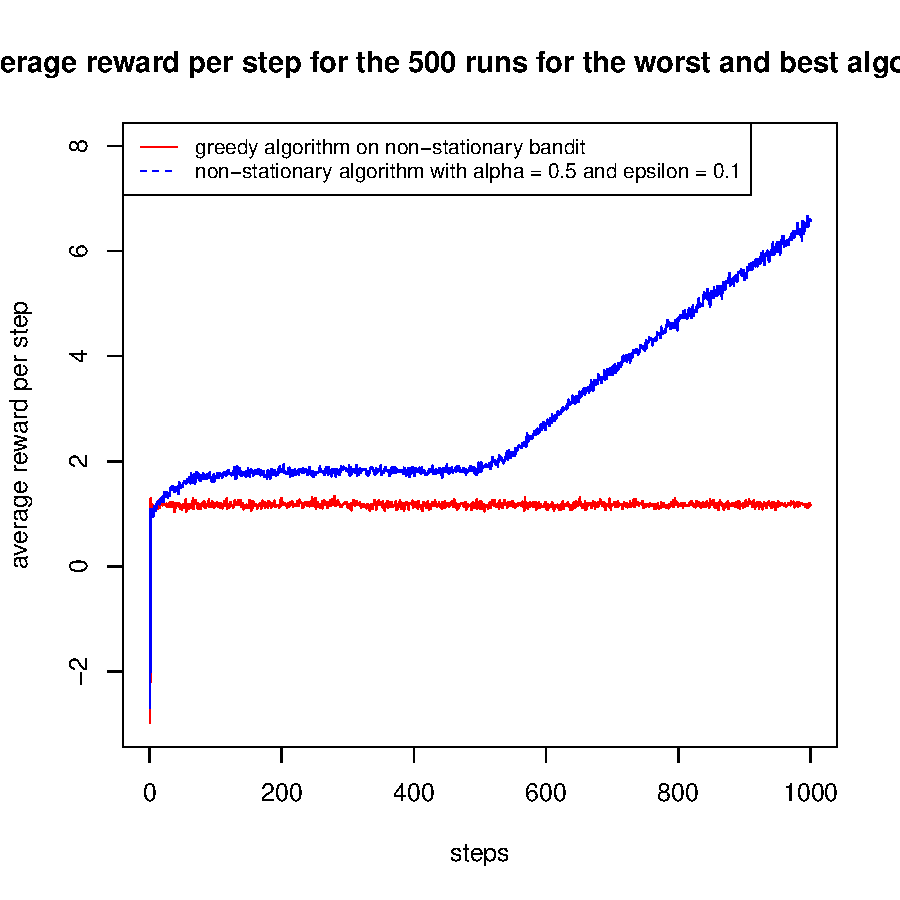
\includegraphics[width=\maxwidth]{figure/unnamed-chunk-12-1} \caption[Average performance of best and worst algorithms]{Average performance of best and worst algorithms}\label{fig:unnamed-chunk-12}
\end{figure}

\end{knitrout}
 



\section{Task 2 Markov Decision Processes}
Here we implement a markov decision process where the agent will do a decision $A_t$ based on the current stat $S_t$ as well as a reward $R_t$, and then return a new state $S_{t+1}$ and a new reward $R_{t+1}$, using the recycling example.

\subsection{Task 2.1: Recycle Robot}
First we use the function for the MDP from the uuml package.


\begin{knitrout}
\definecolor{shadecolor}{rgb}{0.969, 0.969, 0.969}\color{fgcolor}\begin{kframe}
\begin{alltt}
\hlkwd{library}\hlstd{(uuml)}
\hlstd{mdp} \hlkwb{<-} \hlkwd{recycling_mdp}\hlstd{(}\hlnum{0.5}\hlstd{,} \hlnum{0.8}\hlstd{,} \hlnum{0.1}\hlstd{,} \hlnum{1}\hlstd{)}
\end{alltt}
\end{kframe}
\end{knitrout}

\subsection{Task 2.2: always\_search\_policy}
Now to implement a function \texttt{always\_search\_policy} which uses the MPD from the previous task and run the MDP for 1000 steps. The policy is that the agent always chooses to search and it returns the the return divided by the number of time steps and times in each state, and the robot start in the state high. the function \texttt{always\_search\_poliicy} only takes the mdp as an argument, whereas the function \texttt{recycling\_mdp} takes the parameters $\alpha, \beta, \gamma, r_{wait}, r_{search}$ and $n_{steps}$ as arguments.

\begin{knitrout}
\definecolor{shadecolor}{rgb}{0.969, 0.969, 0.969}\color{fgcolor}\begin{kframe}
\begin{alltt}
\hlstd{always_search_policy} \hlkwb{<-}\hlkwa{function}\hlstd{(}\hlkwc{mdp}\hlstd{,} \hlkwc{n_steps}\hlstd{=}\hlnum{1000}\hlstd{)\{}
  \hlcom{#initializing variables}
  \hlcom{#the action will always be search for each iteration}
\hlstd{states} \hlkwb{<-} \hlkwd{c}\hlstd{(}\hlstr{"high"}\hlstd{,} \hlstr{"low"}\hlstd{)}
  \hlstd{N_t} \hlkwb{<-} \hlkwd{c}\hlstd{(}\hlnum{0}\hlstd{,}\hlnum{0}\hlstd{)}
  \hlkwd{names}\hlstd{(N_t)} \hlkwb{<-} \hlstd{states}
  \hlstd{rewards} \hlkwb{<-} \hlkwd{numeric}\hlstd{(n_steps)}
  \hlstd{cur_state} \hlkwb{<-} \hlstr{"high"}
  \hlstd{action} \hlkwb{<-} \hlstr{"search"}

  \hlkwa{for} \hlstd{(i} \hlkwa{in} \hlnum{1}\hlopt{:}\hlstd{n_steps) \{}
    \hlstd{row_index} \hlkwb{<-} \hlkwd{which}\hlstd{(mdp}\hlopt{$}\hlstd{s} \hlopt{==} \hlstd{cur_state} \hlopt{&} \hlstd{mdp}\hlopt{$}\hlstd{a} \hlopt{==} \hlstd{action)}
    \hlstd{p_next} \hlkwb{<-} \hlstd{mdp}\hlopt{$}\hlstd{p_s_next[row_index]}

    \hlstd{state_next} \hlkwb{<-} \hlkwd{sample}\hlstd{(}\hlkwc{x} \hlstd{= states,} \hlkwc{size} \hlstd{=} \hlnum{1}\hlstd{,} \hlkwc{prob} \hlstd{= p_next)}

    \hlstd{N_t[cur_state]} \hlkwb{<-} \hlstd{N_t[cur_state]} \hlopt{+} \hlnum{1}
    \hlstd{reward_index} \hlkwb{<-} \hlkwd{which}\hlstd{(mdp}\hlopt{$}\hlstd{s} \hlopt{==} \hlstd{cur_state} \hlopt{&} \hlstd{mdp}\hlopt{$}\hlstd{a} \hlopt{==} \hlstd{action} \hlopt{&} \hlstd{mdp}\hlopt{$}\hlstd{s_next} \hlopt{==} \hlstd{state_next)}

    \hlstd{rewards[i]} \hlkwb{<-} \hlstd{mdp}\hlopt{$}\hlstd{r_s_a_s_next[reward_index]}

    \hlstd{cur_state} \hlkwb{<-} \hlstd{state_next}
  \hlstd{\}}

  \hlkwd{return}\hlstd{(}\hlkwd{list}\hlstd{(}\hlstr{"Nt"} \hlstd{= N_t,} \hlstr{"R_bar"} \hlstd{=} \hlkwd{mean}\hlstd{(rewards)))}

\hlstd{\}}
\hlkwd{set.seed}\hlstd{(}\hlnum{4711}\hlstd{)}
\hlkwd{always_search_policy}\hlstd{(mdp)}
\end{alltt}
\begin{verbatim}
$Nt
high  low 
 288  712 

$R_bar
[1] 0.452
\end{verbatim}
\end{kframe}
\end{knitrout}

\subsection{Task 2.3: charge\_when\_low\_policy}
Now to implement a function \texttt{charge\_when\_low\_policy} which uses the MPD from the previous task and run the MDP for 1000 steps.
The policy is that the agent always chooses to charge when the state is low and always search if the energy level is high. The function returns the same output structure as the previous function. Hence it is basically the same function, but with an added if statement in the for loop so that the action is not always in search mode. 

\begin{knitrout}
\definecolor{shadecolor}{rgb}{0.969, 0.969, 0.969}\color{fgcolor}\begin{kframe}
\begin{alltt}
\hlcom{#function based on the charge_when_low_policy.}
\hlstd{charge_when_low_policy} \hlkwb{<-}\hlkwa{function}\hlstd{(}\hlkwc{mdp}\hlstd{,} \hlkwc{n_steps}\hlstd{=}\hlnum{1000}\hlstd{)\{}
  \hlcom{#initializing variables}
  \hlstd{N_t} \hlkwb{<-} \hlkwd{c}\hlstd{(}\hlnum{0}\hlstd{,}\hlnum{0}\hlstd{)}
  \hlstd{states} \hlkwb{<-} \hlkwd{c}\hlstd{(}\hlstr{"high"}\hlstd{,} \hlstr{"low"}\hlstd{)}
  \hlkwd{names}\hlstd{(N_t)} \hlkwb{<-} \hlstd{states}
  \hlstd{rewards} \hlkwb{<-} \hlkwd{numeric}\hlstd{(n_steps)}
  \hlstd{cur_state} \hlkwb{<-} \hlstr{"high"}


  \hlkwa{for} \hlstd{(i} \hlkwa{in} \hlnum{1}\hlopt{:}\hlstd{n_steps) \{}
    \hlkwa{if}\hlstd{(cur_state} \hlopt{==} \hlstr{"high"}\hlstd{)\{}
      \hlstd{action} \hlkwb{<-} \hlstr{"search"}
    \hlstd{\}} \hlkwa{else}\hlstd{\{}
      \hlstd{action} \hlkwb{<-} \hlstr{"recharge"}
    \hlstd{\}}
    \hlstd{row_index} \hlkwb{<-} \hlkwd{which}\hlstd{(mdp}\hlopt{$}\hlstd{s} \hlopt{==} \hlstd{cur_state} \hlopt{&} \hlstd{mdp}\hlopt{$}\hlstd{a} \hlopt{==} \hlstd{action)}
    \hlstd{p_next} \hlkwb{<-} \hlstd{mdp}\hlopt{$}\hlstd{p_s_next[row_index]}

    \hlstd{state_next} \hlkwb{<-} \hlkwd{sample}\hlstd{(}\hlkwc{x} \hlstd{= states,} \hlkwc{size} \hlstd{=} \hlnum{1}\hlstd{,} \hlkwc{prob} \hlstd{= p_next)}

    \hlstd{N_t[cur_state]} \hlkwb{<-} \hlstd{N_t[cur_state]} \hlopt{+} \hlnum{1}
    \hlstd{reward_index} \hlkwb{<-} \hlkwd{which}\hlstd{(mdp}\hlopt{$}\hlstd{s} \hlopt{==} \hlstd{cur_state} \hlopt{&} \hlstd{mdp}\hlopt{$}\hlstd{a} \hlopt{==} \hlstd{action} \hlopt{&} \hlstd{mdp}\hlopt{$}\hlstd{s_next} \hlopt{==} \hlstd{state_next)}

    \hlstd{rewards[i]} \hlkwb{<-} \hlstd{mdp}\hlopt{$}\hlstd{r_s_a_s_next[reward_index]}

    \hlstd{cur_state} \hlkwb{<-} \hlstd{state_next}
  \hlstd{\}}

  \hlkwd{return}\hlstd{(}\hlkwd{list}\hlstd{(}\hlstr{"Nt"} \hlstd{= N_t,} \hlstr{"R_bar"} \hlstd{=} \hlkwd{mean}\hlstd{(rewards)))}

\hlstd{\}}
\hlkwd{set.seed}\hlstd{(}\hlnum{4711}\hlstd{)}
\hlkwd{charge_when_low_policy}\hlstd{(mdp)}
\end{alltt}
\begin{verbatim}
$Nt
high  low 
 669  331 

$R_bar
[1] 0.669
\end{verbatim}
\end{kframe}
\end{knitrout}

\subsection{Task 2.4 compare policies}
Lastly we compare the two policies for MDP with $\alpha= \beta = 0.9, and \alpha = \beta = 0.4$ with $r_{\text{wait}} = 0.1, r_{\text{search}} = 1$ and $n_{\text{steps}} = 1000$.

\begin{knitrout}
\definecolor{shadecolor}{rgb}{0.969, 0.969, 0.969}\color{fgcolor}\begin{kframe}
\begin{alltt}
\hlcom{#function that combines both policies given the parameters and returns the R_bar for both policies}
\hlstd{compare_policies} \hlkwb{<-} \hlkwa{function}\hlstd{(}\hlkwc{alpha}\hlstd{,} \hlkwc{beta}\hlstd{,} \hlkwc{r_wait}\hlstd{,} \hlkwc{r_search}\hlstd{,} \hlkwc{n_steps} \hlstd{=} \hlnum{1000}\hlstd{)\{}
  \hlstd{mdp} \hlkwb{<-} \hlkwd{recycling_mdp}\hlstd{(alpha, beta, r_wait, r_search)}
  \hlstd{always_search} \hlkwb{<-} \hlkwd{always_search_policy}\hlstd{(mdp, n_steps)}\hlopt{$}\hlstd{R_bar}
  \hlstd{charge_when_low} \hlkwb{<-} \hlkwd{charge_when_low_policy}\hlstd{(mdp, n_steps)}\hlopt{$}\hlstd{R_bar}
  \hlstd{results} \hlkwb{<-} \hlkwd{c}\hlstd{(always_search, charge_when_low)}
  \hlkwd{names}\hlstd{(results)} \hlkwb{<-} \hlkwd{c}\hlstd{(}\hlstr{"always_search"}\hlstd{,} \hlstr{"charge_when_low"}\hlstd{)}
  \hlkwd{return}\hlstd{(results)}
\hlstd{\}}

\hlstd{replicate_compare_policies} \hlkwb{<-} \hlkwa{function}\hlstd{(}\hlkwc{alpha}\hlstd{,} \hlkwc{beta}\hlstd{,} \hlkwc{r_wait}\hlstd{,} \hlkwc{r_search}\hlstd{,}
                                       \hlkwc{n_steps} \hlstd{=} \hlnum{1000}\hlstd{,} \hlkwc{n_replicates} \hlstd{=} \hlnum{20}\hlstd{)\{}
  \hlstd{multi_results} \hlkwb{<-}\hlkwd{replicate}\hlstd{(n_replicates,}
                            \hlkwd{mapply}\hlstd{(compare_policies,} \hlkwc{alpha}\hlstd{=alpha,} \hlkwc{beta}\hlstd{=beta,}
                                   \hlkwc{r_wait}\hlstd{=r_wait,} \hlkwc{r_search} \hlstd{= r_search,}
                                   \hlkwc{n_steps} \hlstd{= n_steps,} \hlkwc{SIMPLIFY} \hlstd{=} \hlnum{TRUE}\hlstd{),}
                            \hlkwc{simplify} \hlstd{=} \hlnum{FALSE}\hlstd{)}
  \hlcom{#each replication of the mapply returns a table where the rows are the policies}
  \hlcom{#and the columns are the MDPs. Hence multi_results is a list containing}
  \hlcom{#n_replicates number of tables as each element.}

\hlstd{means} \hlkwb{<-} \hlkwd{Reduce}\hlstd{(`+`, multi_results)} \hlopt{/} \hlstd{n_replicates}
\hlkwd{colnames}\hlstd{(means)} \hlkwb{<-} \hlkwd{c}\hlstd{(}\hlstr{"MDP_1"}\hlstd{,} \hlstr{"MDP_2"}\hlstd{)}
\hlkwd{return}\hlstd{(means)}
\hlstd{\}}

\hlkwd{set.seed}\hlstd{(}\hlnum{4711}\hlstd{)}
\hlkwd{replicate_compare_policies}\hlstd{(}\hlkwc{alpha} \hlstd{=} \hlkwd{c}\hlstd{(}\hlnum{0.9}\hlstd{,} \hlnum{0.4}\hlstd{),} \hlkwc{beta} \hlstd{=} \hlkwd{c}\hlstd{(}\hlnum{0.9}\hlstd{,} \hlnum{0.4}\hlstd{),} \hlkwc{r_wait} \hlstd{=} \hlnum{0.1}\hlstd{,}
       \hlkwc{r_search} \hlstd{=} \hlnum{1}\hlstd{,} \hlkwc{n_steps} \hlstd{=} \hlnum{1000}\hlstd{,} \hlkwc{n_replicates} \hlstd{=} \hlnum{15}\hlstd{)} \hlopt
  \hlkwd{round}\hlstd{(}\hlkwc{digits} \hlstd{=} \hlnum{2}\hlstd{)}
\end{alltt}
\begin{verbatim}
                MDP_1 MDP_2
always_search    0.79 -0.20
charge_when_low  0.91  0.63
\end{verbatim}
\end{kframe}
\end{knitrout}

In the output, MDP\_1 corresponds to $\alpha = \beta = 0.9$ and MDP\_2 corresponds to $\alpha = \beta = 0.4$. In general we see that MDP\_1 performs better than MDP\_2. We see that the policy charge\_when\_low\_policy performs better than always\_search\_policy for both $\alpha = \beta = 0.9$ and $\alpha = \beta = 0.4$. The reason for this is that the policy charge\_when\_low\_policy is more efficient, as it only charges when the energy level is low, and therefore it can search more efficiently. The best one was the charge\_when\_low\_policy for $\alpha = \beta = 0.9$ with mean R\_bar = 0.9.

\end{document}

